%!TEX root = thesis.tex
<<<<<<< HEAD
\chapter{Probabilistic Timing Attack against to Snoopy Cache Coherency}
In this chapter of the thesis, we proposed a probabilistic attack to increase evasion probability of malware against to snoopy cache coherence protocol on tightly coupled systems. We briefly explained the issue we can encounter during implementation of the cache oriented obfuscation method. The snoopy cache coherency protocol's internals have already been mentioned in background studies chapter; however, we assumed through whole section that all coherence operations are atomic, and contention between processes are not subject. Yet, They are not close to be atomic; and moreover, the latency is sometimes enough long to process and to complete whole gadget or whole malware. In order to exploit this contention, we methodized a probabilistic race condition attack. 
=======
\chapter{Probabilistic Timing Attack against to Snoopy Cache Coherency Protocol}
In this chapter of the thesis, we proposed a probabilistic attack to increase evasion probability of malware against to snoopy cache coherence protocol on tightly coupled systems. We briefly explained the issue we can encounter during implementation of the cache oriented obfuscation method. The snoopy cache coherency protocol's internals have already been mentioned in background studies chapter; however, assumed through whole section that all coherence operations are atomic, and contention between processes are not subject. Yet, They are not close to be atomic; and moreover, the latency is sometimes enough long to process and to complete whole gadget or whole malware. In order to exploit this contention, we methodized a probabilistic race condition attack. 
>>>>>>> FETCH_HEAD

After we proposed the attack as a solution, we formulated the latency calculation of coherency protocols, compared their variants and enumerated factors which affect latency, and we supported our theories with an acknowledged simulation tool which is written by a team in Stanford University. As it is contention between latency and process overhead, we formulated the calculation of process overhead in it's time interval. As a result, both of these values gives the rate of overall obfuscation , we explained it in the obfuscation rate section. At the end of the chapter, we discussed the attack's feasibility in pitfalls and fallacies section.

As a brief and in other words, instead of giving an absolute obfuscation, we proposed a method which probably obfuscates malware, and this probability depends on the systems design and gadgets' processing overhead. On the other hand, this value gives us a quantitative rate, but if our concern is signature based detection methods, signatures value can be measured with qualitative approaches rather than quantitative ones e.g. some signature like port number or ip address are treasury.  Yet, the quantity of signature is certainly another value to measure efficiency, when especially, we relate binary codes and signature detection.

\section{The Issue}
Cache coherency is a term and discipline arisen from the incoherent states of caches due to parallel computing. It does not need to be multi processing environment. Sometimes, DMA devices can be enough to emerge it. In tightly coupled systems, because of the usage of caches as a private memory, it is highly possible to falling into a incoherency state. We also mentioned much more detail in background studies chapter. in this chapter, the term of "stale data" is used to describe globally\footnote{In local frame, it concerns the relationship between the CPU and cache values rather than between caches. } the data which is not reflected for most current or synchronized value between caches. In order to synchronize stale data and provide coherency between caches, cache coherency protocols and policies are used between caches. As we mentioned, most of  protocols and policies need networks between each other and logical operator per cache controller. There are many methods to provide coherency between caches and one of the most known and capable one is snoop mechanism. 

Snoopy cache coherency mechanisms provide synchronization with a bus watch mechanism in the system bus. These mechanisms imply that cache must first request the data from any other caches, before it request from memory. The implementation of the snoop mechanism is vice versa, but works as same.Cache generally watches the bus and record activities, arise exception in case of coherency problem(when it is likely to fall incoherent states). There is generally an interconnector to organize snoopy cache protocols, and filter useless communication. 

With perfect coherent caches, we can not exploit private caches to use as private memory (see also. NUMA); hence, we can't evade anything from one CPU to another as we did in the previous chapter. Namely, there is no difference between disk to memory and disk to cache obfuscation. Even though the highest workspace which you deobfuscate your code is cache, cache are synchronizing each other. This coherence gives ability to anti-malware scanning other caches and detecting signature.
\section{Solution}
	Let's assume we have a tightly coupled multi processor test bed system, and it has one CPU reserved to scan memory for malware detection, and another CPU is occupied by malware itself. Their caches are snoopy coherent with an interconnection network.  They could use any of protocols which we mentioned in background studies e.g. MOESI, MESI, MSI. Let's also assume that the malware which present in the second CPU's cache is designed as we defined in previous chapter. It has prewarmed cache as we described and started to deobfuscate and run the code. The presumption is the $CACHE 2$`s cache blocks is accessible by $CPU1$ as well as any other CPUs. However, the access and synchronization of any stale data is not that simple. It is presumed as atomic, but it is not, and worst of all, tightly coupled systems are heterogeneous with cache coherency, because the distance to memories are not equal and systems are not homogeneous. This heterogeneousness comes with different access times to the memories. Especially MOESI protocol is much more heterogeneous because it works as semi-NUMA(Non uniform Memory Architecture) type cache i.e. a modified cache block can be moved around various caches without updating main memory. Secondly, cache controllers rule are not really elastic. When an address is touched by a CPU, it fetches whole block in order to exploit spacial locality and increase performance\footnote{Sometimes they wait for feeding CPU until fetch it all, sometimes feed CPU as soon as possible depending on algorithm.}. We actually exploited throughout whole chapter two weaknesses which are horizontal directional cache fetching attribute and synchronization latency and heterogeneous access time of snoopy caches.
\subsection{Horizontal Directional Cache Fetching}
In computer architecture conventions, we arrange instructions into memory space, incrementally, and then, we can prefetch them before they run. Also, we are tent to use the space around we recently accessed. It is called spacial locality and we mentioned about it more deeply in background studies. For this reason, we cache mechanisms works horizontally. It fetches a particular size of memory in the same time, and put it a cache block. Besides, cache blocks are the smallest addressable memory spaces; therefore, it makes caches more simpler, faster\footnote{After an amount of memory, it could decrease performance.\cite{ComputerArchCoursera} }and cheaper. Accordingly, Fetching and eviction operations are handled as line-based namely horizontally. 
	\begin{figure}[h!]
	    \centering
	    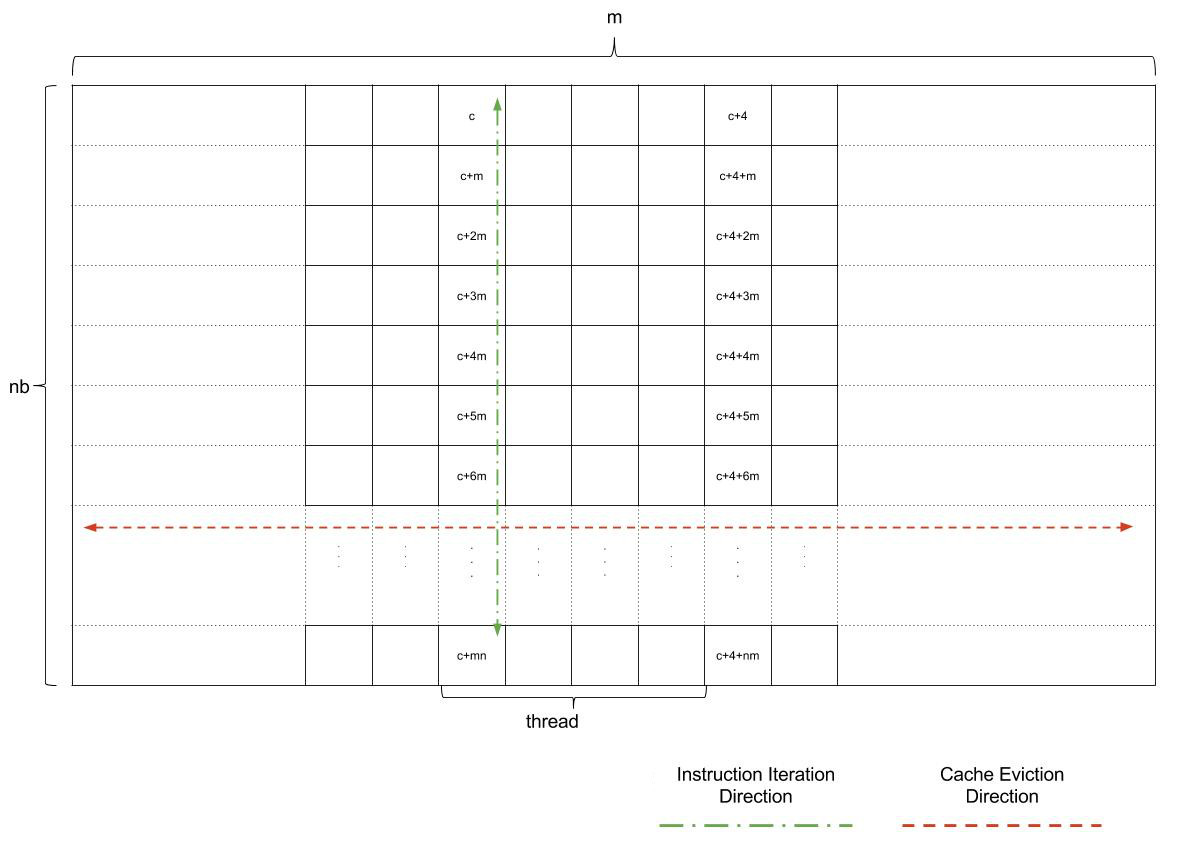
\includegraphics[width=1\textwidth]{img/vertical_instruction_iteration.jpg}
	    \caption{Directional Exploitation}
	    \label{fig:veriticaldirection}
	\end{figure}
In figure \ref{fig:veriticaldirection}, we showed data fetching direction and its contrast with our instruction iteration direction approach. As we mentioned many times, but in order to emphases it one more time, instruction sequence normally increments one by one. Yet, in our approach it iterate as in equation 5.1. $m$ is the cache block size, and $n$ is the number of cache block line in the whole cache. $nb$ is number of line which is allocated to body of our gadget as mentioned in previous chapter, so this figure is a frame of cache in which obfuscated part of our malware allocated. Let's say $c$ is the initialization point of our malware. When $i$ is the number of instruction on the queue, $I(i)$ gives us the location of instruction in the memory; thereby, in the cache. 
\begin{equation}
	I(i)=m*(i\bmod{(nb)})+((\left \lfloor i/nb \right \rfloor*thread)+c)\bmod{m}\\ 
\end{equation}
$thread$ value in the cache is step number between the vertical blocks. In order to generate a function which onto(bijective) the cache frame, equation 5.2 must be provided, because after it overflow mod function, it will uses just the one next block which previously used and go on until end. It is obvious that $tread$ should be smaller than $m$, yet it is already in mod and $i$ must be smaller than total size. 
\begin{equation}
	\forall\: m\bmod thread = 1\ :\  I()\ is\ bijective\ function
\end{equation}
Yet, Why do we iterate institution sequence  vertically? Indeed, we assumed that anti-malware scans horizontally from $CPU1$ above, because it is faster. For example, our code starts from $c$ and our second instruction in $c+m$, with purpose of scanning from $CPU1$ in this order, it should  fetch first the line of $c$ into $Cache2$, and then, it should fetches the line of $c+m$, and so forth. In the perfect world, with atomic instruction to fetches whole cachle line and without latency, it could be race condition free approach, but in real systems, it is not. We will combine this attack with latency problem in next sections.
\subsection{Synchronization Latency of Snoopy Caches}
\subsubsection{Latency Calculation}
2 Latency Calculation Formulas
Interconnector latency relationship
Protocol Latency relationship
1 Table of Systems Latency Comparisons
DOS noise 
\subsubsection*{Simulation Result}
\subsubsection{Process Overhead Calculation}
1 PipeLine Diagram
Out of Order Case
\subsection{The Big Picture}
\subsubsection{Overall Obfuscation Rate Calculation}
\section{Pitfalls and Fallacies}
Deadlock Live Lock
Latecy 
